\chapter{多用户下的可验证对称加密搜索方案研究}
\label{cha:multi-user}
\section{引言}
本章在\single 的基础上,提出了一种适用于多用户场景下的可验证对称加密搜索方案\multi 。该方案同样可以与任意多用户场景下的加密搜索方案结合,来为其提供结果验证功能。与\single 方案不同的是,在多用户的场景下,即数据共享的情况下,数据持有者与数据搜索者产生了分离。数据持有者一方面需要对数据搜索者进行访问控制,以确保数据搜索者只能读取数据而无法写入数据。另一方面,为了保证数据新鲜性,数据持有者还需要在数据发生了更新时,告知数据搜索者。我们将通过公私钥机制解决访问控制问题,并通过时间戳链机制解决数据新鲜性问题。本章的主要内容安排如下:首先介绍了多用户场景下的系统框架,明确了该框架的参与方及所承担的计算任务;随后通过一个抽象定义对该方案工作的流程进行了说明;算法分析部分对抽象定义中的具体算法进行了详细分析;最后,通过安全性分析和实验结果验证了本方案的安全性和有效性。



\section{系统架构}

\begin{figure}[t]
\centering
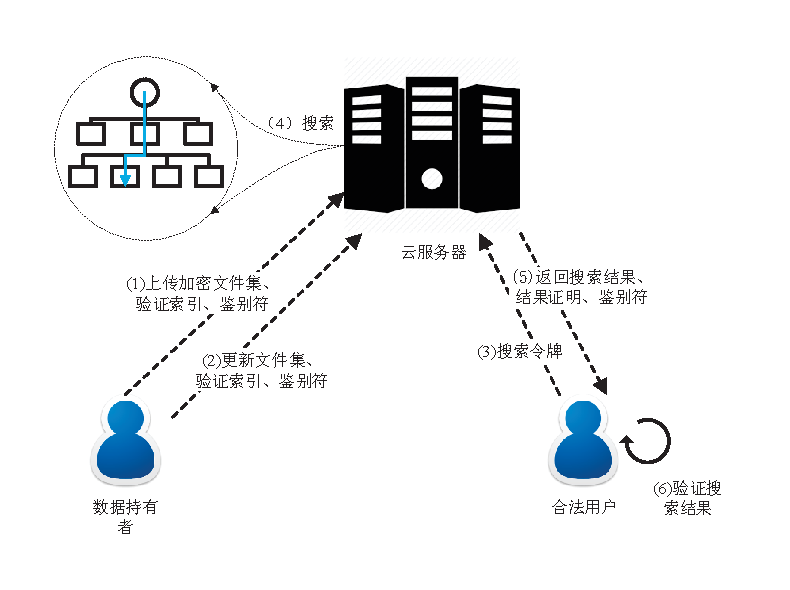
\includegraphics[width=6 in]{fig/GM-VSSE}
\DeclareGraphicsExtensions.
\caption{多用户场景下的可验证对称加密搜索框架\multi}
\label{fig:GM-VSSE}
\end{figure}

多用户场景下的可验证对称加密搜索方案\multi 如图~\ref{fig:GM-VSSE}所示,数据持有者和数据搜索用户产生了分离。首先数据持有者仍然需要对文件集进行处理,得到加密文件集和验证索引,同时他还需要生成一个鉴别符,将三者上传给云服务器。数据持有者在有需要的时候,也需要更新其文件集、验证索引和鉴别符。当一个数据搜索用户被数据持有者授权进行搜索时,他成为了一个合法用户。他可以通过提交搜索令牌来对数据持有者的加密文件集进行搜索。云服务器在收到该搜索令牌以后,需要向其返回加密搜索结果,结果证明以及鉴别符。通过这种方式,我们使得合法用户可以按需获取搜索结果并进行结果验证。


\section{方案流程}
本方案在\single 的基础上进行了改进,旨在为多用户场景下的对称加密搜索方案提供结果验证功能。验证索引的构建仍然需要利用默克尔帕特里夏树和增量哈希技术,同时\multi 方案还使用了时间戳链和公私钥加密体系来实现跨用户的数据新鲜性和数据完整性验证。

\begin{definition}[\textbf{\multi 方案}]\label{def:multi}
  {\itshape
      在 \multi 方案中,参与方有三个, 分别为数据持有者,合法用户以及不可信的云服务器。数据持有者向云服务器提供一个验证索引和鉴别符,是的云服务器可以为合法用户提供搜索结果证明,来确保加密搜索结果的新鲜性和完整性。一个\multi 方案是以下八个算法的集合:
      \begin{itemize}
        \item $KGen(1^k) \rightarrow \{K_1,K_2,K_3, (ssk, spk)\}$: 是由数据持有者执行的秘钥生成算法。它将一个安全参数作为输入,输出对称秘钥 $K_1,K_2,K_3$ 和一对签名公私钥对 $(ssk, spk)$.
        \item $Init(K_1,K_2,K_3, ssk, \mathcal{D}) \rightarrow \{\lambda,\pi\}$: 是由数据持有者执行的初始化算法。它将对称秘钥 $K_1,K_2,K_3$,签名私钥 $ssk$ 和明文文件集 $\mathcal{D}$ 作为输入,输出验证索引 $\lambda$ 和鉴别符 $\pi$。数据持有者在本地保存验证索引$\lambda$的根节点哈希$rt$,并将验证索引$\lambda$和鉴别符 $\pi$上传给云服务器。
        \item $UpdateToken(K_1,K_2,K_3, ssk, d) \rightarrow \{\tau_u, \pi\}$: 是由数据持有者执行的更新令牌生成算法。它将对称秘钥$K_1,K_2,K_3$,签名私钥$ssk$和需要更新的文件$d$作为输入,输出一系列更新令牌$\tau_u$和鉴别符 $\pi$。数据持有者将更新令牌$\tau_u$和鉴别符$\pi$上传给云服务器。
        \item $PreUpdate(\lambda, \tau_u) \rightarrow \{\lambda',\rho_u\}$: 是由云服务器执行的预更新算法。它将验证索引$\lambda$和更新令牌$\tau_u$作为输入,输出更新后的验证索引$\lambda'$和更新证明$\rho_u$。云服务器将更新证明$\rho_u$返回给用户。
        \item $Update(rt,\tau_u,\rho_u) \rightarrow \{rt'\}$:是由数据持有者执行的更新算法。它将验证索引的根哈希 $rt$,更新令牌$\tau_u$和服务器返回的更新证明 $\rho_u$ 作为输入,输出新的根哈希$rt'$。若更新证明$\rho_u$验证通过,则输出更新后的根哈希$rt'$,若更新证明验证失败,则输出的根哈希$rt'$与原始根哈希$rt$相同。
        \item $SearchToken(K_1, w) \rightarrow \{\tau_{w}\}$: 是由数据持有者执行的搜索令牌生成算法。它将对称秘钥$K_1$和某一关键字$w$作为输入,输出与该关键字相关搜索令牌$\tau_{w}$。数据持有者将该搜索令牌 $\tau_{w}$上传给云服务器进行搜索。
        \item $Prove(\lambda, \tau_{w}, t_q) \rightarrow \{\rho,\pi^t_q, \pi_c\}$:是由云服务器执行的结果证明生成算法。它将验证索引$\lambda$,搜索令牌$\tau_{w}$和用户提交查询的时间$t_q$作为输入,输出$\rho$和两个鉴别符$\pi^t_q, \pi_c$作为结果证明。云服务器将结果证明$\rho$,$\pi^t_q, \pi_c$返回给数据搜索用户。
        \item $Verify(K_1,K_2,K_3, spk, C_w, \rho_s, \pi^t_q, \pi_c, \tau_{w},rt) \rightarrow \{b\}$: 是由数据持有者执行的验证算法。它将对称秘钥$K_1,K_2,K_3$,签名公钥$spk$,加密搜索结果$C_w$,结果证明$\rho_s,\pi^t_q, \pi_c$,搜索令牌$\tau_{w}$和保留的验证索引根哈希$rt$作为输入,输出一个比特$b$,代表接受或者拒绝该搜索结果。其中,该算法包括了两个子算法,分别为 $Check$ 算法和 $Generate$ 算法,它们分别可以定义为 $Check(K_3, spk, \pi^t_q, \pi_c) \rightarrow \{b\}$ 和 $Generate(K_1,K_2,K_3,C_w,\rho,\tau_{w},\pi^t_q) \rightarrow \{b\}$.
      \end{itemize}
      }
\end{definition}

\section{具体方案}
本节中,我们将阐述\multi 方案,即多用户场景下的可验证加密搜索框架。注意,由于数据在多个用户之间共享,当数据持有者的数据需要更新时,如何将更新信息同步给多个用户,从而确保数据的新鲜性是本方案的重要挑战。一个简单的想法是,由于验证索引的根哈希是数据新鲜性和数据完整性的保证,在数据持有者需要更新数据时,他只需将更新后的验证索引根哈希值发送给所有的合法用户。但这种方式在数据需要频繁更新的场景下,势必给数据持有者带来巨大的通信开销。并且,这种推送的方法存在带宽浪费,即某些合法用户搜索数据的频率可能较低,在两次推送时间间隔内,并没有数据搜索需求。考虑到该问题,我们提出了一种由合法用户按需获取验证索引根哈希的方式。该方法引入了由时间戳链构造的鉴别符,将验证索引的根哈希值与时间戳绑定,使得用户在搜索数据时,能够获取到最新的根哈希值,用以对数据的新鲜性进行验证。本节的内容安排如下,首先我们将描述如何建立和更新鉴别符,然后我们给出了通过鉴别符验证数据新鲜性的方法,最后通过一个简单的例子介绍了本方案的工作细节。

\subsection{构建及更新时间戳链}
由于云服务器不可信,当数据持有者向云服务器发送了多个鉴别符以后,云服务器有可能会向数据搜索用户重放之前收到的鉴别符,以此来破坏数据新鲜性。针对该问题,本方案采用了时间戳链机制来构造鉴别符,而不仅仅是将验证索引根哈希与时间戳绑定。它使得数据搜索用户可以通过该时间戳链来追踪其中包含的鉴别符,从而确保自身拿到的根哈希值为最新的数据。注意,我们采用的时间戳链方案与可验证对称加密搜索方案~\cite{stefanov2014practical}不同。他们的方案仅仅能在单用户的场景下工作,即在用户持有更新信息的场景下工作。因此,他们的方案不能用户多用户场景下的数据新鲜性验证。

在方案开始工作前,先对方案的设定进行描述,首先数据持有者需要为鉴别符设定一个更新周期 (Update Interval)\footnote{在实验验证环节,我们将展示更新周期与结果验证时延的相关性~\ref{sec:experiments}},即设置固定更新时间点为$\{up_1, up_2, \cdots, up_i, \cdots, up_m\}$。如果更新周期内数据持有者的数据产生了更新,则数据持有者需要生成鉴别符进行上传,否则,数据持有者只需要在固定更新时间点对鉴别符进行上传。
这里我们将使用网络时间协议 (Network Time Protocol, NTP)~\cite{mills1991internet, mills2010network}来对云服务器,数据持有者以及合法用户进行时间同步。注意,时钟同步的精确度目前已经可以达到几毫秒甚至是几十微秒~\cite{kopetz1987clock, elson2002fine, zhou2007accurate},足以保证\multi 方案的验证正确性。此外,一个恶意的云服务器有可能会伪造时钟信息,但他永远无法伪造时间戳链信息,因为时间戳链的信息由数据持有者的秘钥进行了保证。接下来我们将阐释方案细节。

\begin{equation}
  \label{equ:timestamp-chain}
    \left\{
    \begin{array}{ll} % \begin{eqnarray}好像也可以。
      \pi_{i, 0} = (\alpha_{i, 0}, \mathsf{Sig}_{ssk}(\alpha_{i, 0})),~~~~~~~~~~~up_i < tp_{i, 0} \leq up_{i+1} \\
      \alpha_{i, 0} = Enc_{K_3}(rt_{i, 0}||tp_{i, 0}) \\
      \cdots \\

     \pi_{i, j} = (\alpha_{i, j}, \mathsf{Sig}_{ssk}(\alpha_{i, j})),~~~~~~~~~~~tp_{i, j-1} < tp_{i, j} \leq up_{i+1}  \\
     \alpha_{i, j} = Enc_{K_3}(rt_{i, j}||tp_{i, j}||\alpha_{i, j-1}) \\
      \cdots  \\
     \pi_{i, n} = (\alpha_{i, n}, \mathsf{Sig}_{ssk}(\alpha_{i, n})),~~~~~~~~~~~tp_{i, n}=up_{i+1} \\
     \alpha_{i, n} = Enc_{K_3}(rt_{i, n}||tp_{i, n}||\alpha_{i, n-1})
    \end{array}
    \right.
  \end{equation}

\noindent 这里 $i$ 代表第 $i$个更新周期, $j$ 代表该更新周期内的第 $j$个鉴别符.

首先,我们将阐述数据持有者如何通过时间戳链构造鉴别符。
为了防止云服务器重放鉴别符,我们设计了一种基于时间戳链的机制来检测云服务器的恶意行为。我们通过将旧的鉴别符嵌套进新的鉴别符的方式,使得鉴别符串联起来。如公式\ref{equ:timestamp-chain}所示,我们将旧的鉴别符$\pi$与时间戳$tp$和验证索引的根哈希$rt$进行连接,并将联合后的三者用对称秘钥$K_3$加密,同时使用数据持有者的签名私钥$ssk$进行签名,从而生成新的鉴别符。如果验证索引在一个更新周期内没有更新,则数据持有者只需要在下一个固定更新时间点对鉴别符中的时间戳进行更新。如果数据持有者的文件集在更新周期内产生了更新,即验证索引的根哈希产生了更新,则数据持有者需要用更新后的根哈希和最新的时间戳来构建一个新的鉴别符,并上传给云服务器。注意,在每一个更新周期内会行程一个时间戳链,一个时间戳链在下一个更新周期开始时结束,每个时间戳链中的最后一个鉴别符将在下一个固定更新时间点生成。换句话说,每一个更新周期内的鉴别符是连接在一起的,而不同更新周期内的鉴别符是不相关的。

在这种设置下,当一个合法用户发起了一次搜索时,云服务器需要将最新的鉴别符发送给用户。用户可以通过解密鉴别符从其中得到验证索引的根哈希值$rt$和时间戳$tp$。如果时间戳$tp$在最近一次固定更新时间点之前,则可以认为服务器发回了旧的鉴别符,产生了恶意行为。这种方式保证了云服务器无法在最新一次更新周期外产生数据新鲜性攻击。

然而,如果云服务器只传送最新的鉴别符给用户,它仍然可以在最新一次更新周期内产生数据新鲜性攻击。具体地说,如果在最新的更新周期内,数据持有者的文件集产生了一次或者多次的更新,即数据持有者在该更新周期内,上传了多个鉴别符,则云服务器可以发送该更新周期内的任意一个旧的鉴别符来发起数据新鲜性攻击。

为了解决该问题,云服务器除了需要将相对用户搜索时刻的最新鉴别符发送给用户,还需要将一个时间戳链中的最后一个鉴别符发送给用户。我们将距离用户搜索时刻的最近一个时间戳链的结束时间点成为检测点(checkpoint)。通过这种方式,用户可以解密在检测点收到的鉴别符,并使用该鉴别符追踪在搜索时刻收到的鉴别符,以此来判定搜索时刻收到的鉴别符是否为搜索时刻最新的鉴别符,从而防止了云服务器在最新的更新周期内发起数据新鲜性攻击。在下一小节,我们将详细描述用户如何通过两个鉴别符检测云服务器是否发起了数据新鲜性攻击。


\subsection{时间戳验证}
算法~\ref{alg:check}
Algorithm~\ref{alg:check} shows the pseudo-code of the {\it Check} algorithm that is executed by a data user and verifies whether the authenticator has been replayed. Let $\pi^t_q$ denote the authenticator received at the query time $t$ and $\pi_c$ denote the authenticator received at the checkpoint, which is used to deduce the previous authenticators during the latest update interval. First, we need to verify the signature of $\pi^t_q$ and $\pi_c$ by using the public key $spk$ of the data owner. We check the authenticator $\pi^t_q$ received at the query time is not generated before the previous update time point by using $\alpha^t_q$ extract from $\pi^t_q$. Then, we decrypt the previous $rt_k||tp_k||\alpha_{k-1}$ concatenation by using $\alpha_k$ until it finds the first concatenation with timestamp $tp_k < t$ or $\alpha_k = \emptyset$. We compare $\alpha_k$ with $\alpha^t_q$ and $\emptyset$. If it is not equal to either of them, a data freshness attack is detected. Otherwise, $\alpha^t_q$ is considered correct.

\begin{algorithm}[t]
  \caption{Check}
  %\setcounter{algorithm}{2.1}
  \label{alg:check}
  \begin{algorithmic}[1]
    \REQUIRE {$K_3$: the symmetric key; $spk$: the public key for verifying signature; $\pi^t_q$: the authenticator received in the query time $t$; $\pi_c$: the authenticator received in the checkpoint.}
    \ENSURE {$b \in \{0,1\}$, if $b=1$, the {\it Check} algorithm succeeds, otherwise, it fails.}
              \STATE{let $\pi^t_q = \{\alpha^t_q, Sig^t_q\}$ and $\pi_c = \{\alpha_c, Sig_c\}$}
              \IF{$\alpha^t_q \neq (Sig^t_q)_{spk}$ $\vert \vert$ $\alpha_c \neq (Sig_c)_{spk}$}
                \RETURN{$b = 0$}
              \ENDIF
              \STATE {$(rt^t_q, tp^t_q, \alpha) \leftarrow Dec_{K_3}(\alpha^t_q)$}
              \IF{$tp^t_q$ is not before the previous update time point}
                \STATE {let $\alpha_k = \alpha_c$}
                \FOR {$\alpha_k \neq \emptyset$}
                    \STATE {$(rt_k, tp_k, \alpha_{k-1}) \leftarrow Dec_{K_3}(\alpha_k)$}
                    \IF {$tp_k < t$}
                      \BREAK
                    \ENDIF
                    \STATE {let $\alpha_k = \alpha_{k-1}$}
                \ENDFOR
                \IF {$\alpha_k = \alpha^t_q ||\alpha_k = \emptyset$}
                  \RETURN {$b = 1$}
                \ELSE
                  \RETURN {$b = 0$}
                \ENDIF
              \ELSE
                \RETURN {$b = 0$}
              \ENDIF
  \end{algorithmic}
\end{algorithm}

\noindent \textbf{Remark.} The update interval can be controlled by the data owner according to its update frequency. Normally, if data is frequently updated, the update interval can be set to a shorter period so that the length of the authenticator will decrease and the verification delays will be shorter. However, it will incur more communication overheads.
%However, if the update is not frequent, the update interval can be set longer to reduce the bandwidth consumption introduced by the fixed update.
% incurred by the fixed update point.
In our experiments (see Section~\ref{sec:experiments}), we will show that the verification delays and the bandwidth consumption for updating authenticators are acceptable.

\subsection{实例分析}

\begin{figure}[htb]
  \centering
  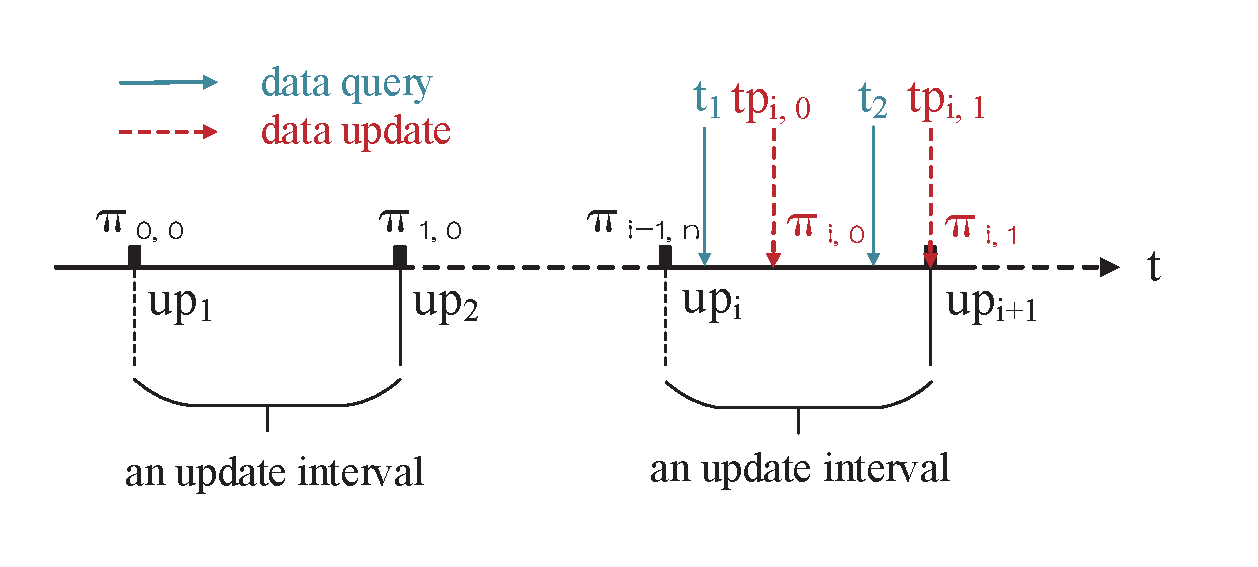
\includegraphics[width=6 in]{fig/timestamp}
  \DeclareGraphicsExtensions.
  \caption{An illustration of the timestamp-chain mechanism}
  \label{fig:timestamp}
\end{figure}

the authenticators in each update interval are chained together, e.g., $\pi_{i, 0}, \pi_{i, 1}$ (see Fig.~\ref{fig:timestamp}),but the authenticators are irrelevant in the two different update intervals.

the checkpoint is referred as the next update time point closest to the user's query time $t$, e.g., $up_{i+1}$ is the checkpoint in the update interval $(up_i,up_{i+1}]$.


Let us consider the following cases (shown in Fig.~\ref{fig:timestamp}) when a data user initiates a query at different time points: (i) the first case is that the query occurs at $t_1$, where $t_1 < tp_{i, 0}$, the server can only send $\pi_{i-1, n}$ to the data user; (ii) the second case is that the query occurs at $t_2$ after the data update event at $tp_{i, 0}$, and the authenticator that server sends to the user is $\pi_{i, 0}$; (iii) the last case is that the query is generated at $t_2$, and the authenticator sent by the server is $\pi_{i-1, n}$. In the last case, a data freshness attack occurs, but it will be detected at the checkpoint $up_{i+1}$. The data user will obtain the last authenticator $\pi_{i, 1}$ from the server at the checkpoint to verify whether the data obtained at the query time has been replayed or not.

Now we use the three cases above to explain the algorithm. In the first case, $\pi_{i, 1}$ and $\pi_{i, 0}$ are received and $\alpha_{i,1}$ and $\alpha_{i,0}$ are extracted. We can find the field of $\alpha$ in the concatenation is $\emptyset$ after decrypting $\alpha_{i, 0}$. Therefore, the {\it Check} algorithm outputs $b=1$ and the authenticator $\pi_{i-1, n}$ received in the query time is considered correct. In the second case, $\alpha_{i, 0}$ is also decrypted by $\alpha_{i, 1}$ and the timestamp of $\alpha_{i, 0}$ is less than $t_2$. We can find that $\alpha_{i, 0}$ and $\alpha^{t_2}_q$ are equal. Hence $\alpha^{t_2}_q$ is considered correct, i.e., $\pi^{t_2}_q$ is correct. However, in the last case, we will detect a data freshness attack due to the mismatch between the correct authenticator $\pi_{i, 0}$ and the received one $\pi^{t_2}_q$, i.e., $\pi_{i-1, n}$.

\section{安全性分析}

\section{实验结果}
\label{sec:experiments}
\begin{figure}[ht]
  \begin{minipage}[b]{0.49\textwidth}
    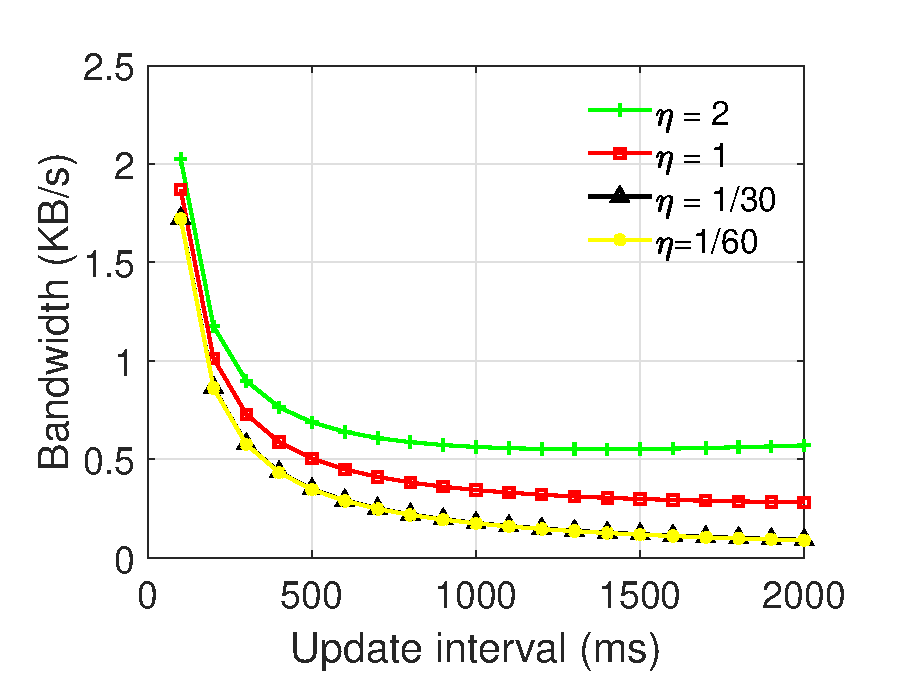
\includegraphics[width= 3 in]{expr/bandwidth}
    \caption{带宽开销}
    \label{fig:bandwidth}
  \end{minipage}
  \begin{minipage}[b]{0.49\textwidth}
    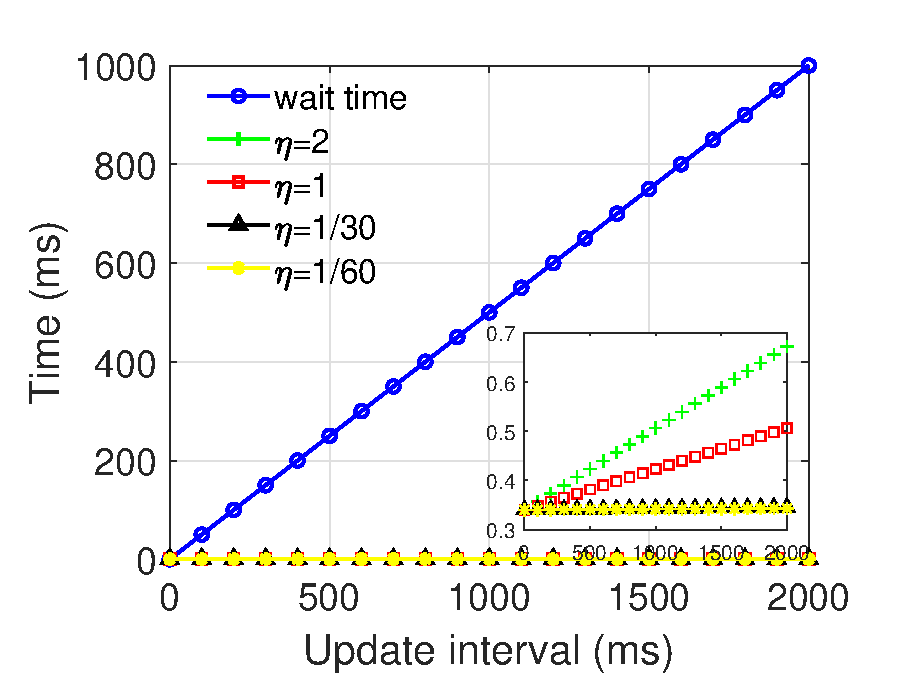
\includegraphics[width= 3 in]{expr/verify-2}
    \caption{总验证时间开销}
    \label{fig:verify-2}
  \end{minipage}
\centering
\end{figure}


In Fig.~\ref{fig:verify-2}, we evaluate the verification delays in data users. Note that an entire verification delay includes the delay of waiting for a checkpoint and the delay of executing the {\it Check} and the {\it Generate} algorithms. Since the execution delay of the {\it Generate} algorithm is relatively stable, around 0.1 milliseconds, we do not plot it in Fig.~\ref{fig:verify-2}. Here, $\eta$ is the update frequency of the data owner. We assume that the time that a user initiates a query is uniformly distributed during an update interval, and then the user's waiting delays are also uniformly distributed. Therefore, the expected delay is half of the update interval and the verification delays are dominated by the waiting delays. The execution delay of the {\it Check} algorithm is negligible and is proportional to the update interval, which is mainly incurred by verifying the signature and decrypting authenticators.
Kindly note that in above measurement, we do not take into account the network transmission and propagation delays, as they vary in different specific network contexts and do not reflect the essential extra cost directly introduced by our verification design. We do, however, report the communication overhead in terms of the message size, as shown in Fig.~\ref{fig:bandwidth}. In a later experiment, we will also show that we can set an update interval so as to make a trade-off between verification delays and communication overhead.

Fig.~\ref{fig:bandwidth} shows the bandwidth costs for authenticator update. %Here, $b$
Here, the size of the first authenticator in each update interval is around 112 bytes, which includes 32 bytes of the root of MPT, 8 bytes of the timestamp, an 8 bytes AES-CBC extension and a 128 bytes RSA signature. Overall, the bandwidth of the authenticator includes two part: the overhead introduced by the fixed update time point and the overhead introduced by data update. We can observe that the bandwidth cost increases to about 2KB per second when the update interval decrease to zero, this is introduced by the fixed update time point which is inversely proportional to the bandwidth overhead. Moreover, the bandwidth gradually increases when the update interval becomes too long. This overhead is introduced by the length of the authenticator, because as the update interval grows, the length of the authenticator becomes larger. Overall, the cost should be acceptable to achieve \multi. According to the results, in order to make a decent tradeoff between verification delays and bandwidth costs, we suggest choosing an update interval between 500 milliseconds and 1,500 milliseconds.

图9和图10评估了系统的总验证开销,包括计算开销和通信开销。我们主要考虑合法用户端的验证计算开销,和数据拥有者端的通信开销。图中的η表示数据拥有者的数据更新频率。
首先,我们考虑合法用户端的验证开销。这部分开销包括用户等待检测点的时间以及执行Check算法和Rebuild算法的时间。由于Rebuild算法的开销可以忽略,因此图9中并未标注该部分开销。如图9所示,蓝色的曲线表示合法用户等待检测点的时间,这里我们假设合法用户的查询时刻在一个更新周期内呈均匀分布,那么用户等待时间的均值就是更新间隔的一半。其余的曲线表示Check算法的执行时间,可以看到,当更新频率在2Hz到1/60Hz不等时,Check算法的执行时间也几乎可以忽略,因此合法用户端的验证开销主要取决于等待检测点所需的时间,即和更新间隔的设置有关。
其次,我们考虑数据拥有者端的通信开销。我们主要考虑由鉴别符带来的开销。由于鉴别符的更新包含两种情况,固定更新导致的鉴别符更新和数据更新导致的鉴别符更新。图10中的曲线充分体现了这两种更新带来的开销。首先,当数据拥有者的更新间隔设置的很小时,通信开销较大,这是因为固定更新太频繁导致的鉴别符的通信开销增大;当数据拥有者的更新间隔设置的很大时,通信开销也较大,这是因为当更新频率一定时,更新间隔越大,在更新间隔内形成的鉴别符的长度会累积增大,最终导致了鉴别符的通信开销增大。
综合以上两种情况,更新间隔可以设置为1000ms至1500ms之间。
